\phantomsection

\chapter{Referencial Teórico}

O presente capítulo apresenta os conceitos teóricos necessários para o desenvolvimento do princípio de funcionamento do dispositivo.
São apresentados tópicos referentes a solicitações mecânicas e resistência dos materiais, princípios de sensoriamento de deformação e instrumentação de extensômetros,
obtenção de sinais e transmissão de dados. Também será apresentado as principais tecnologias necessárias para o processo de desenvolvimento do dispositivo.

\section{SOLICITAÇÕES E RESISTÊNCIA DOS MATERIAIS}

Um entendimento introdutório sobre resistência dos materiais é necessário de modo a entender sobre os comportamentos físicos de um componente mecânico
que sofre a ação de cargas externas. O ponto de partida do estudo da resistência dos materiais é o da análise do comportamento mecânico de um componente em equilíbrio.

Utilizando as equações de estática, deve-se determinar as forças e os momentos resultantes que agem no interior de um corpo, com a finalidade de verificar
e garantir a integridade do mesmo durante o uso \autocite{Hibbeler2010}. Um corpo em equilíbrio, deve satisfazer a \autoref{eq:Eq_110} e \autoref{eq:Eq_120}, que
descrevem o balanço estático conforme a segunda lei de Newton.

\begin{equation}\label{eq:Eq_110}%
\mbox{\fontsize{17.28}{21.6}\selectfont\( %
\sum F_{x} = \sum F_{y} = \sum F_{z} = 0
\)} %
\end{equation}

\begin{equation}\label{eq:Eq_120}%
\mbox{\fontsize{17.28}{21.6}\selectfont\( %
\sum M_{x} = \sum M_{y} = \sum M_{z} = 0
\)} %
\end{equation}

%onde
%
%$F_{i}$: Forças axiais aplicadas no corpo no eixo "i"
%
%$M_{i}$: Momentos aplicados no corpo no eixo "i"

\hfill

Para ser mantida a condição de equilíbrio do corpo do material sobre forças externas devem estar presentes forças e momentos internos ao seu corpo.
Uma das mais importantes aplicações da estática na análise de problemas de resistência dos materiais é poder determinar os esforços internos
presentes em um, esses esforços são necessários para manter sua integridade submetido a cargas externas, onde as forças e os momentos que agem em um
ponto específico do corpo representam os efeitos resultantes da distribuição dessas forças no local \autocite{Hibbeler2010}.
A \autoref{fig:1010} apresenta uma representação gráfica da atuação de forças internas em um material:

\begin{figure}[htb]
	\caption{\label{fig:1010} Forças internas atuando em um corpo em equilíbrio}
	\begin{center}
		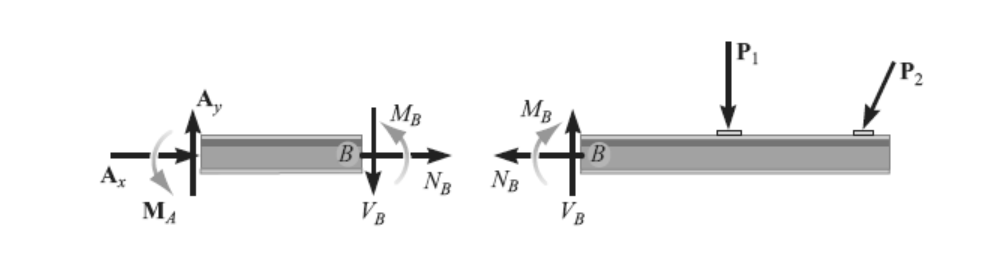
\includegraphics[width=\textwidth]{pictures/1010.jpg}
	\end{center}
	\fonte{https://pressbooks.library.upei.ca/statics/chapter/3-types-of-internal-forces/ acesso em mar 2022}
\end{figure}

Uma vez que se tem a informação das forças internas atuantes em um ponto no corpo e na seção do material, então, pode-se partir para a análise das tensões
e deformações do local de análise.

\subsection{Deformação e limites do material}

Quando um segmento de um corpo sob balanço estático se encontra sob a ação de forças internas, este segmento apresentará uma variação de comprimento e forma relativos
á forças aplicadas. Deformação é definido como a mudança de comprimento por unidade de comprimento, logo, é um valor adimensional,
e é calculada pela \autoref{eq:Eq_130} \autocite{Norton2011}.

\begin{equation}\label{eq:Eq_130}%
\mbox{\fontsize{17.28}{21.6}\selectfont\( %
\varepsilon = \frac{l - l_0}{l_0}
\)} %
\end{equation}

%onde
%
%$\varepsilon$: Deformação presente no material
%
%$l$: Comprimento da barra após deformação
%
%$l_0$: Comprimento da barra sem deformação

\hfill

Com o objetivo de descobrir os limites no qual um material pode-se deformar antes de sua ruptura devem ser analisados seus diagramas tensão-deformação.
Hibbeler ressalta a importância na análise desse tipo de diagrama, uma vez que eles proporcionam meios para a obtenção de dados sobre resistência à tração
ou compressão de um material independentemente das características geométricas em que é utilizado \autocite{Hibbeler2010}.
Um exemplo de diagrama tensão-deformação é mostrado na \autoref{fig:1020}.

\begin{figure}[htb]
	\caption{\label{fig:1020} Exemplo de diagrama tensão-deformação}
	\begin{center}
		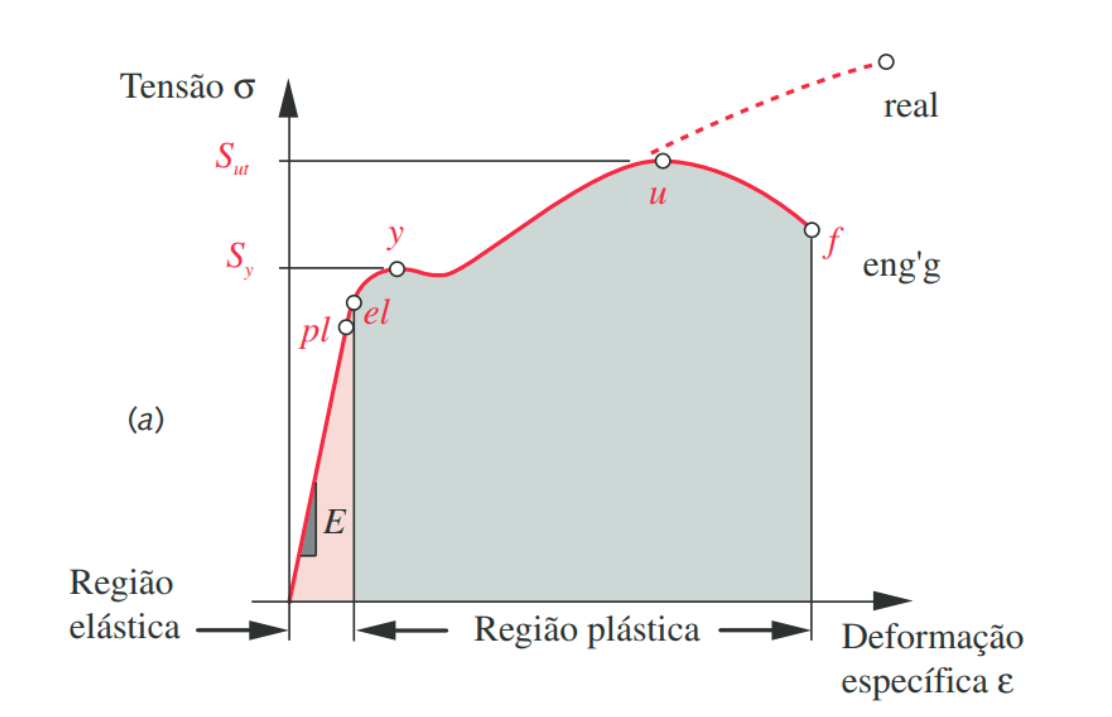
\includegraphics[width=\textwidth]{pictures/1020.png}
	\end{center}
	\fonte{\autocite{Norton2011}}
\end{figure}

Analisando o diagrama anterior pode-se notar uma zona de relacionamento linear entre a força aplicada no corpo de prova e sua deformação,
nesta região é observado o comportamento de deformação elástica do material e sobre seu limite.
Para aplicações de engenharia os pontos $pl$ e $el$ do diagrama são considerados os mesmos devidos á sua proximidade, este ponto representa
o limite entre o comportamento elástico e plastico do material. \autocite{Norton2011}

Na maior parte dos materiais de engenharia é verificada uma relação linear entre deformação e tensão dentro da região elástica, logo, um aumento
nas forças externas aplicadas em um material resultam em um aumento proporcional das deformações locais caso a condição de tensão esteja dentro
do limite elástico, esse fato foi descoberto por Robert Hooke, em 1676, em molas e é conhecido como Lei de Hooke \autocite{Hibbeler2010}.
A lei de Hooke é apresentada na \autoref{eq:Eq_140}.

\begin{equation}\label{eq:Eq_140}%
\mbox{\fontsize{17.28}{21.6}\selectfont\( %
\sigma = E \varepsilon
\)} %
\end{equation}

%onde
%
%$\sigma$: Tensão interna do material
%
%$E$: Módulo de elasticidade do material
%
%$\varepsilon$: Deformação presente no material

\hfill

A variável $E$ da equação da Lei de Hooke é representa a inclinação da curva tensão-deformação e é chamada de Módulo de Young, ou módulo de elasticidade do
material \autocite{Norton2011}. Norton também afirma que o Módulo de Young “é uma medida da rigidez do material em sua região elástica e tem as mesmas unidades da tensão.
A maioria dos metais exibe esse comportamento linear e também tem módulos de elasticidade que variam muito pouco com tratamentos térmicos ou com a adição de elementos de liga.”

Para uma barra constituída de um material homogêneo e isotrópico e submetida a forças axiais que tem seu centro de atuação no centro da seção da barra essas cargas
irão gerar uma tensão normal uniforme ao longo do seu comprimento sobre a seção transversal \autocite{Hibbeler2010}.

\begin{figure}[htb]
	\caption{\label{fig:1030} Deformação de uma barra sob carga de tração}
	\begin{center}
		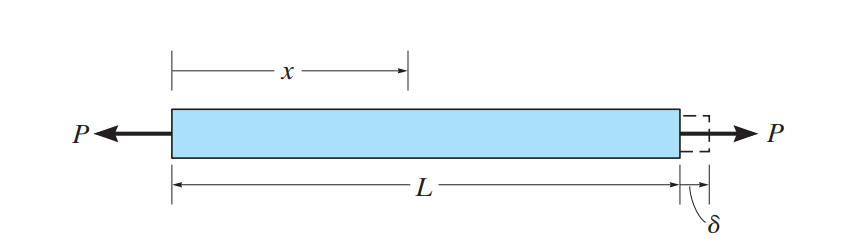
\includegraphics[width=\textwidth]{pictures/1030.png}
	\end{center}
	\fonte{\autocite{Hibbeler2010}}
\end{figure}

O alongamento ou contração de um segmento de reta por unidade de comprimento é denominado deformação normal e segue a \autoref{eq:Eq_150}.

\begin{equation}\label{eq:Eq_150}%
\mbox{\fontsize{17.28}{21.6}\selectfont\( %
\delta = \frac{PL}{AE}
\)} %
\end{equation}

%onde
%
%$\delta$: Variação de comprimento na barra
%
%$P$: Carga aplicada
%
%$A$: Área da seção transversal
%
%$L$: Comprimento da barra

\hfill

%Para outros tipos de carregamentos também são notados valores de deformação relativos às cargas aplicadas, os principais utilizados no desenvolvimento do experimento são introduzidos não sub subseções abaixo.

%% todo REVIEW
%
% \subsection{Deformação de um eixo em torção}
%
%Eixos normalmente são utilizados em situações em que as cargas torcionais são consideráveis, e caso estejam presentes cargas normais ou de flexão em sua utilização, e o material encontra-se em balanço estático, pode-se utilizar as mesmas equações de deformação da análise de barras e vigas.
%\autocite{Norton2011} afirma que “quando barras são solicitadas por um momento em relação ao seu eixo longitudinal, diz-se que estão sob torção, esse tipo de momento aplicado é denominado torque e esta situação é comum em eixos que transmitem potência.” A deformação vista no corpo de um eixo sob cargas de torção pura ao longo da sua seção transversal é ilustrada na \autoref{fig:1040}.
%
%\begin{figure}[htb]
%	\caption{\label{fig:1040} Representação do efeito da deformação em um eixo sob torção}
%	\begin{center}
%		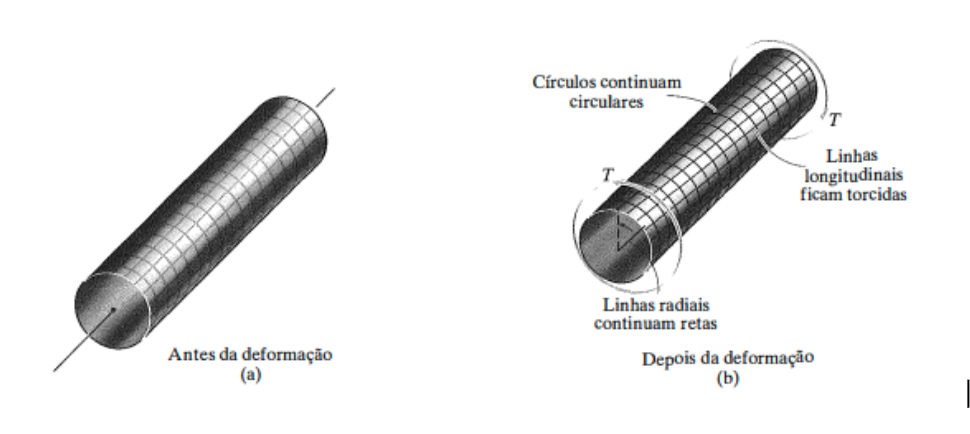
\includegraphics[width=\textwidth]{pictures/1040.png}
%	\end{center}
%	\fonte{\autocite{Hibbeler2010}}
%\end{figure}
%
%A Lei de Hooke para um corpo sob forças de torção é semelhante a mesma para o caso de um corpo em tração ou compressão como apresentada na \autoref{eq:Eq_160}.
%
%\begin{equation}\label{eq:Eq_160}%
%\mbox{\fontsize{17.28}{21.6}\selectfont\( %
%\tau = \frac{Gr\theta}{l_0}
%\)} %
%\end{equation}
%
%%onde
%%
%%$\tau $: Tensão torcional no material
%%
%%$G$: Módulo de elasticidade torcional
%%
%%$r$: raio da seção transversal
%%
%%$\theta$: Ângulo de deformação
%%
%%$l_0$: Comprimento do material
%
%\hfill
%
%Desta vez o módulo presente dessa vez é denominado módulo de elasticidade transversal $G$ que é definido em termos do módulo de elasticidade $E$ e do coeficiente de Poisson $\nu$ do material.
%O coeficiente de Poisson $\nu$ representa a relação entre a deformação específica lateral e longitudinal do material.\autocite{Norton2011}
%
%\begin{equation}\label{eq:Eq_170}%
%\mbox{\fontsize{17.28}{21.6}\selectfont\( %
%G = \frac{E}{2(1+\nu )}
%\)} %
%\end{equation}
%
%%onde
%%
%%$G$: Módulo de elasticidade torcional
%%
%%$E$: Módulo de elasticidade do material
%%
%%$\nu$: Módulo de Poisson do material
%
%\hfill
%
%A \autoref{tab:PoissonValues} apresenta os principais valores de coeficiente de Poisson para diferentes materiais metálicos. \autocite{Norton2011}
%
%\begin{table}[h]
%    \caption{Valores de coeficiente de Poisson para os principais materiais metálicos}
%    \label{tab:PoissonValues}
%    \centering
%    \resizebox{150}{!}{%
%        \begin{tabular}{ l | r } \toprule
%            Material & $\nu$ \\\hline
%            Alumínio & ${0.34}$ \\
%            Cobre & ${0.35}$ \\
%            Ferro & ${0.28}$ \\
%            Aço & ${0.28}$ \\
%            Magnésio & ${0.33}$ \\
%            Titânio & ${0.34}$ \\
%            \bottomrule
%        \end{tabular}}
%\fonte{O autor 2022}
%\end{table}
%
%Assim como visto na \autoref{fig:1040} é notado que a deformação nessa situação não se apresenta como aumento de comprimento do componente, como no caso da uma barra sob cargas axiais, mas por uma distribuição de deslocamentos angulares locais na direção radial da seção do eixo conforme se aumenta a dimensão de comprimento da análise das cargas internas como apresentado na \autoref{fig:1050}.
%
%\begin{figure}[htb]
%	\caption{\label{fig:1050} Deformação e distribuição de tensão em um eixo sob torção}
%	\begin{center}
%		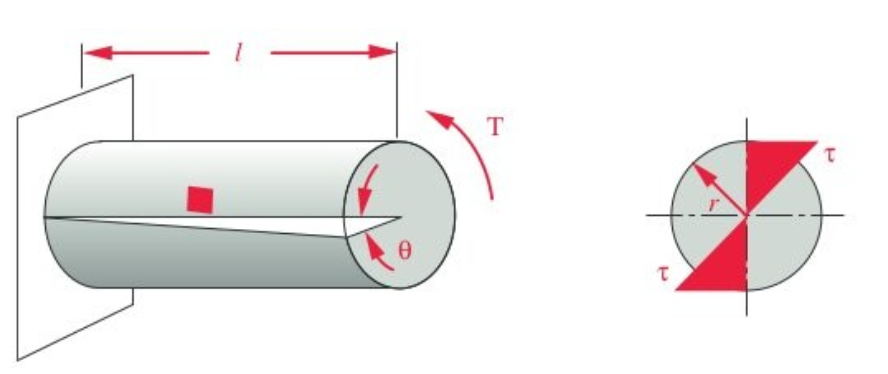
\includegraphics[width=\textwidth]{pictures/1050.png}
%	\end{center}
%	\fonte{\autocite{Norton2011}}
%\end{figure}
%
%A \autoref{eq:Eq_180} é obtida da análise da Lei de Hooke para um eixo em torção.
%
%\begin{equation}\label{eq:Eq_180}%
%\mbox{\fontsize{17.28}{21.6}\selectfont\( %
%\theta = \frac{Tl}{GJ}
%\)} %
%\end{equation}
%
%\hfill
%
%\begin{equation}\label{eq:Eq_190}%
%\mbox{\fontsize{17.28}{21.6}\selectfont\( %
%\tau = \frac{Tr}{J}
%\)} %
%\end{equation}
%
%%onde
%%
%%$T$: Torque aplicado no eixo
%%
%%$r$: Raio da seção transversal
%%
%%$l$: Comprimento do eixo
%%
%%$G$: Módulo torsional de elasticidade
%%
%%$J$: Momento polar de inércia
%
%\hfill
%
%Assim como as barras em tração, as equações aqui apresentadas apenas consideram a operação do componente em regime de deformação elástico, logo os valores esperados de θ serão relativamente pequenos para materiais de engenharia.
%
%% todo END REVIEW

\subsection{Deformação de uma viga em flexão}

A flexão é presente em um corpo sempre que as forças não são aplicadas na direção normal da sua seção transversal.
O momento fletor é causado pelas cargas externas que tendem a fletir o corpo em torno do eixo perpendicular ao plano da
área da seção transversal do material, e esse momento tende a produzir uma variação linear da tensão normal ao longo da
seção de uma viga. \autocite{Hibbeler2010}
A \autoref{fig:1060} mostra uma representação ilustrativa do efeito do momento fletor em uma viga.

\begin{figure}[htb]
	\caption{\label{fig:1060} Representação do efeito da deformação em uma viga sob flexão}
	\begin{center}
		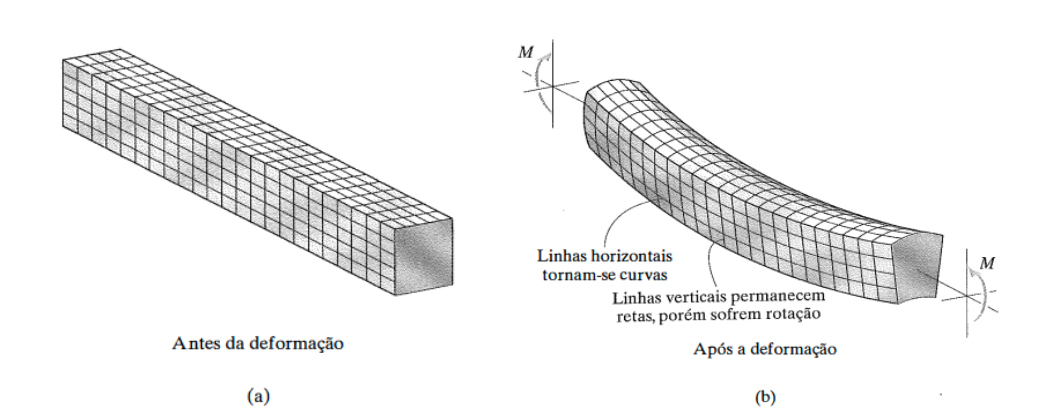
\includegraphics[width=\textwidth]{pictures/1060.png}
	\end{center}
	\fonte{\autocite{Hibbeler2010}}
\end{figure}

Em todo caso em que o material seja homogêneo e isotrópico e que a Lei de Hooke seja aplicável, pode-se relacionar o momento fletor presente com a distribuição de
tensão na seção, como mostrado na \autoref{fig:1070}. Assim como a barra em torção, a tensão, e eventualmente a deformação presente será função da distância entre o
ponto de análise e o centro da área da seção transversal do material \autocite{Hibbeler2010}.
A \autoref{eq:Eq_200} caracteriza a distribuição de tensão ao longo da seção do componente.

\begin{figure}[htb]
	\caption{\label{fig:1070} Deformação e distribuição de tensão em uma sob flexão}
	\begin{center}
		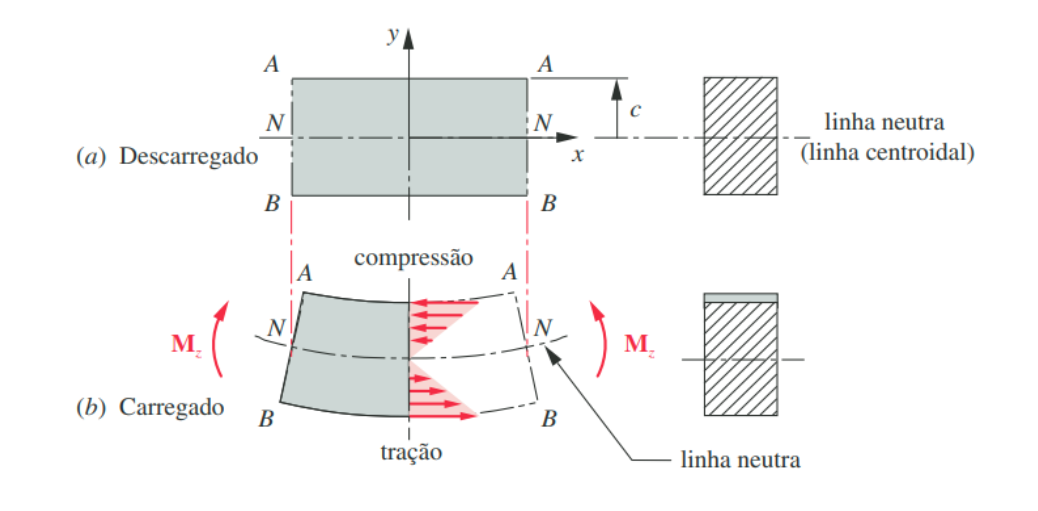
\includegraphics[width=\textwidth]{pictures/1070.png}
	\end{center}
	\fonte{\autocite{Norton2011}}
\end{figure}

\begin{equation}\label{eq:Eq_200}%
\mbox{\fontsize{17.28}{21.6}\selectfont\( %
\sigma = - \frac{My}{I}
\)} %
\end{equation}

%onde
%
%$M$: Momento fletor
%
%$I$: Momento de inércia da seção transversal
%
%$y$: Distância entre limite da área e seu centroide
%

\hfill

O valor de $I$ representa o momento de inércia da seção do material sobre carga de flexão e a variável $y$ representa a distância entre o centroide da seção transversal
e o ponto de análise de tensão. Deve-se notar que as tensões máximas para qualquer corpo em flexão sempre acontecerão na superfície do material, e que enquanto um ponto
qualquer está sob forças de tração, o ponto simétrico a este estará sob forças de compressão.
Uma vez conhecido o módulo de elasticidade do material e a distribuição de tensão na seção de um corpo sob flexão, pode-se obter, utilizando a lei de Hooke, os valores
de deformação na superfície causados pelas cargas de flexão.

As deformações em um componente podem ser altamente visíveis ou praticamente imperceptíveis se não forem utilizados equipamentos que façam medições precisas
\autocite{Hibbeler2010}. Considerando essa afirmação deve-se também ser estudado o método experimental de obtenção de dados de deformação nos componentes.

\section{EXTENSOMETRIA}

O extensômetro de resistência elétrica é o dispositivo mais utilizado para medir a deformação em uma superfície.
O princípio de funcionamento desse tipo de sensor é baseado no efeito de variação de resistência elétrica de um condutor quando
ocorre uma variação de área da sua seção transversal \autocite{Hollman2011}.

Caso um extensômetro esteja fixado a um corpo de um material em uma direção específica, como na \autoref{fig:1080} qualquer carga que deforma a superfície desse corpo de prova irá
deformar igualmente o extensômetro, logo pode-se considerar o extensômetro como uma parte integrante do corpo de prova e qualquer deformação que aconteça no corpo de
prova acontecerá igual no extensômetro \autocite{Hibbeler2010}.

\begin{figure}[htb]
	\caption{\label{fig:1080} Extensômetro fixado á um corpo de prova}
	\begin{center}
		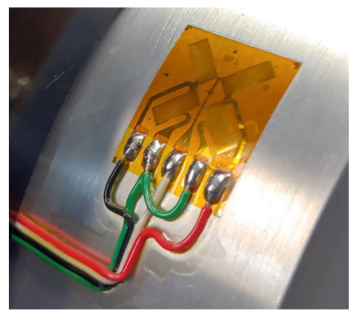
\includegraphics[width=\textwidth]{pictures/1080.png}
	\end{center}
	\fonte{https://binsfeld.com/category/strain-gage/ acesso em fev 2022}
\end{figure}

O fator de extensão ou gage factor, parâmetro que especifica a relação entre a variação da resistência nominal em um extensômetro para um valor unitário
de deformação, é um valor especificado pelo fabricante, então, e a resistência nominal do extensômetro são valores especificados pelo fabricante do sensor,
então, medindo um valor e variação de resistência elétrica no extensômetro pode-se obter um valor de deformação local \autocite{Hollman2011}.
A \autoref{eq:Eq_210} mostra uma relação entre a variação de resistência elétrica no extensômetro e os parâmetros repassados pelo fabricante.

\begin{equation}\label{eq:Eq_210}%
\mbox{\fontsize{17.28}{21.6}\selectfont\( %
k \varepsilon = \frac{\Delta R_s }{R_s}
\)} %
\end{equation}

%onde
%
%$k$: Gage Factor
%
%$\varepsilon$: Deformação no extensômetro
%
%$\Delta R_s$: Variação de resistência causada pela deformação
%
%$R_s$: Resistência nominal do extensômetro
%
%\hfill

Porém, deve-se notar que os valores de deformação esperados para um metal dentro de sua zona de deformação elástica são muito pequenos, o que acarreta em pequenas
variações de resistência no extensômetro. Com o objetivo de facilitar a medição da deformação, devem ser utilizados artifícios de instrumentação como um circuito de ponte
com a finalidade de detectar com maior sensibilidade as variações de resistência do sensor.

\subsection{Ponte de Wheatstone}

Circuitos de ponte são utilizados para prover melhores medições e precisões em uma variedade de aplicações de medição de resistência elétrica, indutância e capacitância
sob condições tanto estáticas quanto transientes.
Dentre diversos tipos de circuitos de ponte a ponte de Wheatstone, mostrada na \autoref{fig:1090}, é um dos tipos de circuito elétrico
mais utilizado para facilitar a leitura da variação de resistência de sensores que apresentam baixas variações de resistência elétrica na sua operação \autocite{Hollman2011}.

\begin{figure}[htb]
	\caption{\label{fig:1090} Ponte de Wheatstone}
	\begin{center}
		
\includegraphics[width=300]{pictures/1090.png}
	\end{center}
	\fonte{https://www.researchgate.net/figure/Monolithic-integration-of-a-Wheatstone-bridge-circuit-with-the-paper-based-sensor-A_fig2_224225141\\ acesso em fev 2022}
\end{figure}

A ponte de Wheatstone é normalmente utilizada em comparações e medições de resistência elétrica que variam de 1 $\Omega$ até 1 $M\Omega$ \autocite{Hollman2011}.
A \autoref{eq:Eq_220} é obtida utilizando as leis de kirchhoff para obter o valor de tensão entre pontos B e D.

\begin{equation}\label{eq:Eq_220}%
\mbox{\fontsize{17.28}{21.6}\selectfont\( %
V_{out} = V_{in} \frac{R_1 R_3 - R_2 R_4}{(R_1 + R_2)(R_3 + R_4)}
\)} %
\end{equation}

%onde
%
%$V_{out}$: Tensão de saída da ponte
%
%$V_{in}$: Tensão de excitação da ponte
%
%$R_i$: Resistência nominal dos resistores da ponte

\hfill

Em uma aplicação onde o sensor de deformação representa uma resistência variável dentro do circuito e os outros resistores apresentam resistências
iguais ao do valor nominal do sensor utilizado, pode-se combinar a equação prévia com a equação do fator de extensão para obter uma relação entre tensão obtida
e valor de extensão apresentado no sensor, logo a equação de transferência do circuito é representada na \autoref{eq:Eq_225}.

\begin{equation}\label{eq:Eq_225}%
\mbox{\fontsize{17.28}{21.6}\selectfont\( %
\frac{V_{out}}{V_{in}} = \frac{k}{4}(\varepsilon_1 - \varepsilon_2 + \varepsilon_3 - \varepsilon_4)
\)} %
\end{equation}

%onde
%
%$V_{out}$: Tensão de saída da ponte
%
%$V_{in}$: Tensão de excitação da ponte
%
%$k$: Gage factor
%
%$\varepsilon_{i}$: Valor de deformação no extensômetro "i"

\hfill

Circuitos de ponte se mostram de grande utilidade em experimentos práticos e são amplamente utilizados na medição da resistência de transdutores como extensômetros
e outros tipos de sensores que convertem uma grandeza física em uma variação de resistência. Para medições estáticas, a tensão de saída do circuito de ponte é normalmente
medido utilizando um voltímetro ou um dispositivo de coleta de dados de tensão \autocite{Hollman2011}.

Uma vez conhecido o fato de que não aconteceram grandes variações de tensão em um extensômetro na sua operação, devido ao fato do material apresentar pequenos valores de
deformação dentro de sua zona elástica, pode-se concluir que o sinal de saída da ponte de Wheatstone ainda não apresentará altos valores de tensão, logo, deve-se estudar métodos de
amplificação dessa tensão com o objetivo de facilitar a obtenção das leituras por um voltímetro digital ou placa de controle.

\section{OBTENÇÃO DE SINAIS}

Medidas experimentais podem ocorrer de diversas formas e em vários casos os sinais são considerados fracos, logo eles devem ser amplificados com o objetivo de facilitar sua
utilização por um dispositivo de saída. A maior parte dos amplificadores de sinal atuais utilizam circuitos integrados ou dispositivos de estado sólido para amplificar um
sinal fraco analógico \autocite{Hollman2011}.

\begin{figure}[htb]
	\caption{\label{fig:1100} Princípio de funcionamento de um amplificador de sinal}
	\begin{center}
		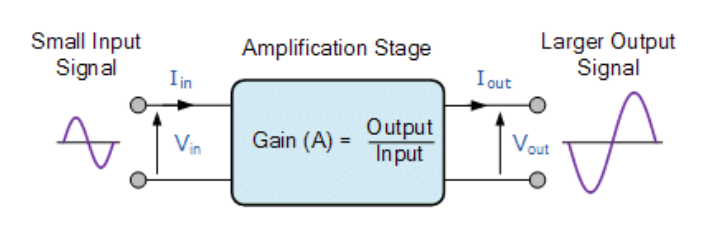
\includegraphics[width=\textwidth]{pictures/1100.png}
	\end{center}
	\fonte{https://www.electronics-tutorials.ws/amplifier/amp_1.html\\ acesso em fev 2022}
\end{figure}

O principio de funcionamento de um amplificador de sinal é mostrado na \autoref{fig:1100}.
O grau de amplificação de um amplificador pode ser dado pela \autoref{eq:Eq_230}, que relaciona o sinal de entrada recebido pelo amplificador de sinal com o sinal de saída, que é lido pelo controlador.

\begin{equation}\label{eq:Eq_230}%
\mbox{\fontsize{17.28}{21.6}\selectfont\( %
Gain(A) = \frac{input}{output}
\)} %
\end{equation}

%onde
%
%$Gain (A)$: Grau de amplificação do amplificador de sinal
%
%$input$: Sinal de entrada
%
%$output$: Sinal amplificado

\hfill

Ruídos característicos sempre estarão presentes em situações de tomada de medidas, como ilustrado na \autoref{fig:1110}.
Os ruídos acontecem devido a efeitos aleatórios ou conhecidos e podem ser filtrados utilizando circuitos que apenas permitem que uma certa parte das frequências que compõem o sinal obtido passem
adiante no circuito a fim de modificar o sinal de saída do amplificador.
Essa filtragem dos ruídos não resolvem todos os problemas que podem ser encontrados, porém melhora significativamente o resultado de um experimento \autocite{Hollman2011}.

\begin{figure}[htb]
	\caption{\label{fig:1110} Ilustração de ruídos presentes em sinais analógicos e digitais}
	\begin{center}
		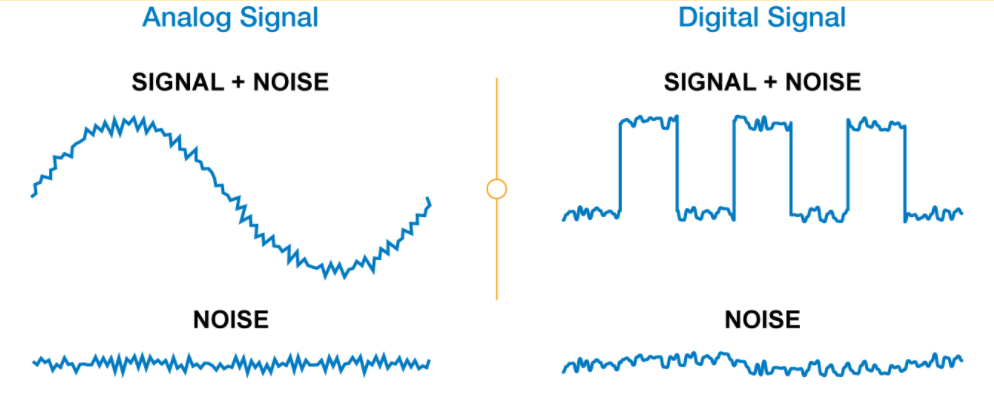
\includegraphics[width=\textwidth]{pictures/1110.png}
	\end{center}
	\fonte{www.quora.com/How-can-digital-signals-posses-noise-immunity acesso em fev 2022}
\end{figure}

Uma vez que os sinais encontrados até aqui no sistema são de característica analógica e espera-se que a utilização e tratamento deles ocorra em um computador ou placa
controladora como o ESP32, que opera de maneira digital, deve-se então converter essas informações de tensão de um meio analógico para um meio digital, para isso é utilizado
um conversor digital-analógico.
Em um meio analógico, as variáveis físicas são processadas como valores num meio contínuo, enquanto em um meio digital, valores são caracterizados por uma representação
discreta, como ilustrado na \autoref{fig:1120}.

\begin{figure}[htb]
	\caption{\label{fig:1120} Representação gráfica de um sinal analógico em forma digital}
	\begin{center}
		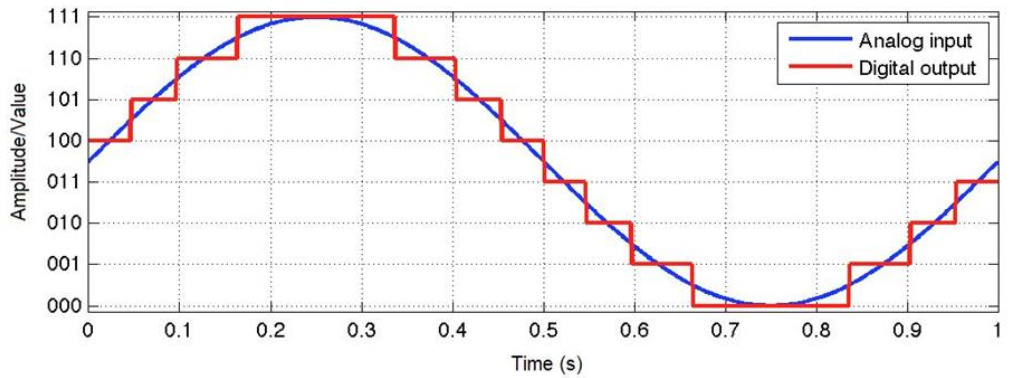
\includegraphics[width=\textwidth]{pictures/1120.png}
	\end{center}
	\fonte{{www.arrow.com/en/research-and-events/articles/engineering-resource-basics-of-analog-to-digital-converters} acesso em fev 2022}
\end{figure}

Uma daz razões para o tratamento de sinais de maneira digital é amenizar o efeito de ruídos durante a transmissão do sinal devido ao fato de que valores no meio discreto
são menos sensíveis a ruídos por possuírem apenas dois valores de estados possíveis, 0 ou 1.
Em contrapartida os sinais analógicos são muito mais sensíveis a ruídos pois podem apresentar uma infinidade de valores possíveis dentro de um meio contínuo,
logo, qualquer ruído pode alterar os valores transmitidos dos sinais \autocite{Hollman2011}.

Com a finalidade de não ser perdidas informações no momento de conversão de um sinal do meio analógico para a forma digital, deve ser seguido o teorema sampling que estipula
que a taxa de leitura de um sinal de maneira digital necessita ser pelo menos duas vezes o valor da frequência desse sinal no meio analógico \autocite{Hollman2011}.

A aquisição e processamento subsequente dos sinais obtidos pode ser feito de diversas formas, desde simples cálculos e obtenção manuais de dados até utilizando
rotinas computacionais complexas. O objetivo do sistema de aquisição de dados é o de coletar, processar e/ou armazenar os dados obtidos em um experimento ou medição
\autocite{Hollman2011}.

\section{SISTEMAS DE MEDIÇÃO}

A maior parte dos sistemas de medição podem ser divididos em três estágios principais, um estágio de detecção da medida física, um estágio intermediário tratamento de sinal e um estágio final,
que engloba o processamento do sinal por um dispositivo de controle e a apresentação dos resultados por um observador \autocite{Hollman2011}.
Uma representação esquemática de um sistema de medição genérico é ilustrado na \autoref{fig:1130}.

\begin{figure}[htb]
	\caption{\label{fig:1130} Diagrama de blocos dos estágios de um sistema de medição}
	\begin{center}
		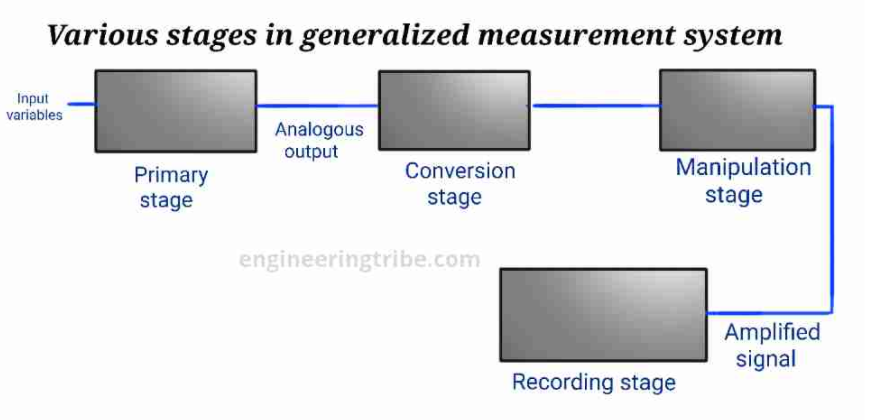
\includegraphics[width=\textwidth]{pictures/1130.png}
	\end{center}
	\fonte{O autor 2022}
\end{figure}

Uma medição é considerada estática quando a grandeza física analisada não apresenta mudanças no tempo.
Um exemplo de medição estática seria a análise da deformação superficial de uma viga sob a ação de uma carga constante de flexão.
Se o tipo de carregamento do exemplo fosse de forma cíclica ou apresentasse vibrações consideráveis, então não pode mais se considerar o sinal como sendo estático \autocite{Hollman2011}.

Para desenvolver o sistema de controle e obtenção do sinal foi utilizado a plataforma de desenvolvimento ESP32, mostrado na \autoref{fig:1140}.
Suas principais vantagens sobre a plataforma Arduino, que é mais amplamente utilizada, é devido ao fato de que o ESP32 apresenta em sua construção módulos de comunicação sem fio bluetooth
e wireless integrados, o que eventualmente reduz complexidade e preço do dispositivo por não ser necessária a utilização de um módulo de comunicação externo \autocite{DocsESP32}.

\begin{figure}[htb]
	\caption{\label{fig:1140} Controlador ESP32}
	\begin{center}
		
\includegraphics[width=\textwidth]{pictures/1140.jpg}
	\end{center}
	\fonte{amazon.com}
\end{figure}

A programação do controlador é feita utilizando uma linguagem de programação baseada na linguagem C + + adaptada para a utilização em placas de controle utilizando o ambiente
de desenvolvimento Arduino IDE, que permite a utilização de extensões para programação e utilização de módulos externos, como o amplificador de sinal.

O ADS1115 é um conversor analógico digital, mostrado na \autoref{fig:1150}.
É um módulo de precisão com amplificador de ganho programável, e que tem resolução de 16 bits.
O módulo é capaz de obter sinais na frequência de até 860 amostras por segundo e consegue sensoriar sinais na faixa de tensão de ${\pm 256}{m\V}$,
isso permite o sensoriamento de sinais de baixa energia com alta resolução \autocite{DocsADS115}.

\begin{figure}[htb]
	\caption{\label{fig:1150} Conversor analógico digital ADS1115}
	\begin{center}
		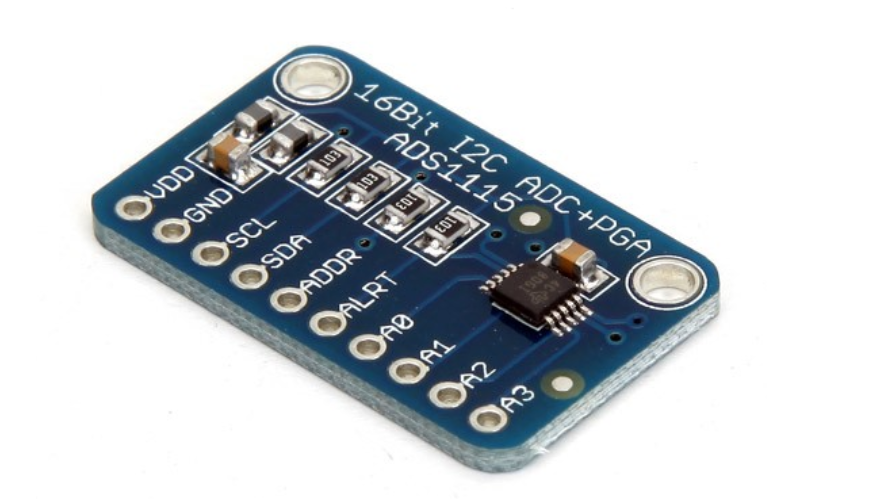
\includegraphics[width=\textwidth]{pictures/1150.png}
	\end{center}
	\fonte{amazon.com}
\end{figure}

Os dados obtidos pelo sistema de medição são todos em formato digital em forma de vetores unidimensionais compostos pelos valores das amostras obtidas durante o tempo do
experimento, esses valores são transmitidos em tempo real para um computador que executa um programa de obtenção de dados para realizar transformações mais complexas e
análises dos sinais obtidos em tempo real.

\section{ANÁLISE DOS SINAIS OBTIDOS}

Algum tipo de análise deve sempre ser feita em todo tipo de conjuntos de dados experimentais. Várias considerações entram na determinação final da validade dos resultados
experimentais, erros podem acarretar na invalidade dos dados mesmo quando estes foram obtidos com cautela. Alguns erros são de natureza aleatória, e outros podem ser por
natureza física ou por descuido do experimentador, como flutuações eletrônicas, fricção ou desgaste dos componentes, esses tipos de erros devem ser descartados imediatamente
\autocite{Hollman2011}.

Leituras individuais em um instrumento podem variar devido a erros de natureza aleatória, que seguem uma distribuição estatística normal, e o experimentador pode estar
desejando obter o valor médio de diversas leituras realizadas \autocite{Hollman2011}. A \autoref{eq:Eq_240} obtém o valor médio para uma medição experimental consistente
de diversas leituras.

\begin{equation}\label{eq:Eq_240}%
\mbox{\fontsize{17.28}{21.6}\selectfont\( %
\overline{x} = {\frac {1}{n}}\sum _{i=1}^{n}x_{i}
\)} %
\end{equation}

%onde:
%
%$\overline{x}$: Valor médio das amostras
%
%$x_i$: valor nominal da amostra i
%
%$n$: Quantidade de amostras

\hfill

Para cada leitura é esperado um valor de desvio lido, deve se notar que quanto melhor for o sistema de medição menor serão os valores de desvio obtidos no conjunto de
leituras, o desvio padrão, representado pela \autoref{eq:Eq_250}, se mostra como um bom indicador da situação dos desvios, e consequentemente da exatidão de um sistema de
medição.

\begin{equation}\label{eq:Eq_250}%
\mbox{\fontsize{17.28}{21.6}\selectfont\( %
Dp = \sqrt{\frac{\Sigma(x_i-\overline{x})^{2}}{n}}
\)} %
\end{equation}

%onde:
%
%$Dp$: desvio padrão
%
%$x_i$: valor nominal da amostra "i"
%
%$\overline{x}$: valor médio das amostras
%
%$n$: Quantidade de amostras

\hfill

Essa equação de desvio padrão deve ser utilizada para grandes populações de amostras ou para quando os dados obtidos podem ser comparados com grandezas conhecidas \autocite{Hollman2011}.
Para se obter a informação de se os valores experimentais estão de acordo com os desejados pode-se utilizar o teste do chi quadrado, representado na \autoref{eq:Eq_260}.

\begin{equation}\label{eq:Eq_260}%
\mbox{\fontsize{17.28}{21.6}\selectfont\( %
\chi^{2} = \sum{\frac{(observed_i - expected_i)^{2}}{expected_i}}
\)} %
\end{equation}

%onde:
%
%$\chi^{2}$: valor de chi quadrado
%
%$observed$: valor experimental observado da amostra "i"
%
%$expected$: valor experimental esperado da amostra "i"

\hfill

Esse teste é uma importante ferramenta de teste de qualquer resultado de distribuição experimental esperada. Se o valor de chi quadrado é igual a zero
então a distribuição assumida é exatamente a distribuição real, quanto maior o valor de chi quadrado, menor é a correlação entre os dados medidos e os reais. \autocite{Hollman2011}

\subsection{Ambiente de desenvolvimento computacional Python}

A linguagem computacional Python é utilizada tanto para desenvolvimento do software que realiza a comunicação entre o sistema de medição e o computador durante a utilização,
quanto para a criação de rotinas para obtenção dos dados estatísticos para cada amostra obtida.

Python é uma linguagem de programação de alto nível com sintaxe simples de fácil leitura e entendimento.
É possível a utilização de extensões e pacotes com funções pré desenvolvidas para resolver diversos problemas computacionais encontrados pelos programadores \autocite{TimHall2010}.

Uma das extensões principais que é utilizado neste trabalho é o Requests, que é um pacote com funções que tem como objetivo simplificar as operações de requisição e obtenção de dados entre dispositivos
que se encontram conectados á uma mesma rede, seja ela uma rede local ou na rede mundial de computadores \autoref{DocsRequests}.

A extensão Numpy é um pacote fundamental para computação científica utilizando a linguagem de programação Python.
O Numpy é uma ferramenta utilizada para o processamento de dados em forma vetorial, uni ou multidimensional, seu funcionamento é baseado na conversão dos dados numéricos do formato de lista para um
formato específico, altamente otimizado chamado ndarray.
O pacote Numpy também apresenta diversas funções matemáticas, lógicas, estatísticas, algébricas feitas para serem utilizadas com objetos ndarray, isso acarreta na maior facilidade de programação e
na minimização de processamento de um programa se comparado com a utilização de funções nativas de Python \autocite{DocsNumPy}.

%As principais funções utilizadas são demonstradas na \autoref{tab:PythonNumpy}.

%\begin{table}[htb]
%	\caption{Funções do pacote NumPy utilizadas}
%	\label{tab:PythonNumpy}
%	\resizebox{\textwidth}{!}{%
%		\begin{tabular}{p{2.0cm}p{5.0cm}p{3.0cm}p{3.0cm}}
%			\toprule
%			\textbf{Função} & \textbf{Descrição } & \textbf{Parâmetros de entrada} & \textbf{Parâmetros de saída} \\
%			\midrule
%			array & Cria um objeto do numpy & Lista python & Vetor ndarray \\
%			average & Obtem valor médio & Vetor ndarray & Valor médio \\
%			std & Obtém desvio padrão & Vetor ndarray & Valor desvio padrão \\
%			amax & Obtém valor máximo & Vetor ndarray & Valor máximo \\
%			amin & Obtém valor mínimo & Vetor ndarray & Valor mínimo \\
%			\bottomrule
%		\end{tabular}
%	}
%	\fonte{O autor (2022)}
%\end{table}

Uma grande gama de outros pacotes em python usam como base a estrutura de dados e funções presentes, como o Pandas, que é utilizado para facilitar a manipulação e
armazenamento de dados em formato de tabular, como planilhas e bancos de dados \autocite{DocsPandas}.
Dados em formatos tabulares do Pandas podem facilmente ser processados, analisados e armazenados utilizando funções do Numpy e funções nativas do Pandas.

Com o auxílio do processamento de dados tabulares e utilizando as funções estatísticas do pacote Numpy pode-se facilmente obter os valores nominais e de erro de cada medida
tomada com o dispositivo de medição.

%\subsection{Análise dos valores nominais}
%
%Uma vez obtidos todos os valores nominais para cada situação experimental analisada, devem ser criadas representações gráficas da distribuição dos resultados obtidos para
%isso é utilizado o pacote scipy, que é uma coleção de algoritmos matemáticos e funções de conveniência, desenvolvidos em cima do pacote Numpy. Ele proporciona ao usuário
%funções e classes para manipulação e visualização de dados científicos. O pacote scipy se mostra como um forte competidor aos ambientes de desenvolvimento mais comumente
%utilizados, como o Matlab, Scilab e o Octave \autocite{DocsSciPy}.
%
%A principal visualização a ser obtida no experimento é o gráfico de distribuição de cargas aplicados pelos valores de tensão da ponte de Wheatstone obtidos, então, utilizando
%o método de minimização dos quadrados, pode-se obter os parâmetros básicos que descrevem uma função matemática em que os erros entre valores observados do experimento e os
%estimados sejam o mínimo o possível.
%
%\begin{figure}[htb]
%	\caption{\label{fig:1160} Regressão linear}
%	\begin{center}
%		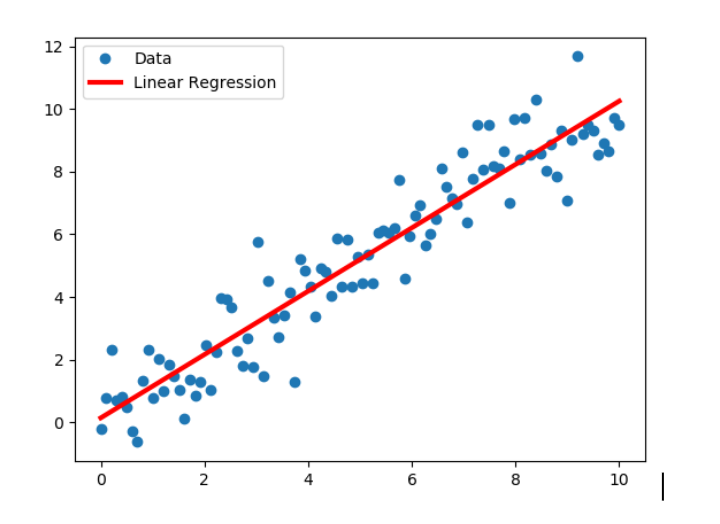
\includegraphics[width=\textwidth]{pictures/1160.png}
%	\end{center}
%	\fonte{www.researchgate.net/figure/Linear-Regression-model-sample-illustration_fig3_340271573 acesso em fev 2022}
%\end{figure}
%
%O gráfico de regressão linear dos dados experimentais é obtido utilizando a função scipy.lialg.regress do pacote scipy.

\section{METODOLOGIA DE DESENVOLVIMENTO DE PROJETO DE PRODUTO}

Desenvolvimento de produto entende-se como o processo de transformação de informações e conceitos até a produção e uso de um produto. Para se desenvolver um novo produto
é necessário saber o que fazer, para quem fazer, quando fazer, com que fazer e como fazer. Esta organização é denominada metodologia de projeto ou metodologia de
desenvolvimento de produtos. \autocite{Back2008}

O projeto de um produto engloba todas as etapas de definição das funções e características operacionais necessárias em um produto a ser desenvolvido, o modelo PRODIP
divide o projeto em macro etapas, cada uma contemplando uma fase do desenvolvimento de um produto, uma visão geral das etapas dessa metodologia é mostrada na \autoref{fig:1170}.
\autocite{PRODIP}.

\begin{figure}[htb]
	\caption{\label{fig:1170}Etapas da metodologia PRODIP}
	\begin{center}
		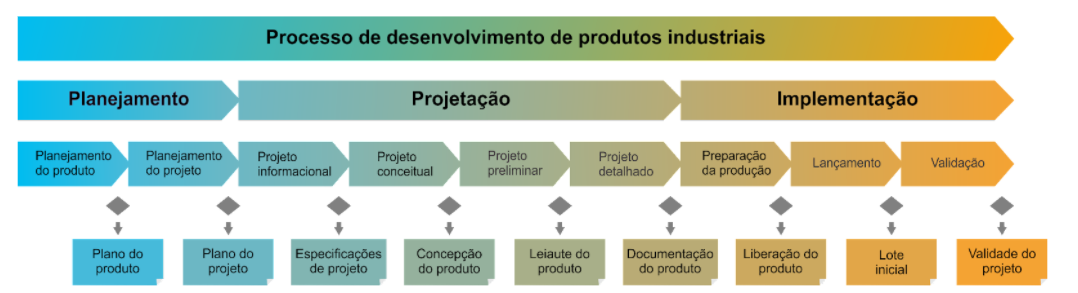
\includegraphics[width=\textwidth]{pictures/1170.png}
	\end{center}
	\fonte{\autocite{PRODIP}}
\end{figure}

Novos produtos não precisam ser necessariamente produtos totalmente originais.
Um produto novo pode ser obtido pela atualização, melhorias e/ou modificações de um produto existente, desta forma um produto existente pode ser reintroduzido a um novo
nicho de mercado, e ele será considerado um novo produto.
Para problemas de pequeno porte, pode ocorrer de que não exista a necessidade de se seguir um longo e rigoroso caminho para o desenvolvimento do projeto do produto \autocite{Back2008}.

Embasado no argumento indicado por Back em sua obra, a metodologia seguida segue as etapas apresentadas na metodologia PRODIP, porém, nem todas as ferramentas e sub etapas
apresentadas serão rigorosamente seguidas, neste trabalho o autor simplifica as macro etapas do projeto devido ao fato que o resultado final deste não será o de um produto
em estado de produção em massa.

\subsection{Fase de planejamento}

A fase de planejamento do projeto visa definir as etapas de desenvolvimento das ideias selecionadas utilizando definições de escopo.
Nesta etapa são definidas as ideias de problema e do produto, um mapeamento tecnológico, e organizadas as informações de mercado, produto e tecnologias, que são correlacionadas
e servem de base para estabelecer o plano do produto \autocite{PRODIP}.

O resultado da fase de planejamento do projeto é um documento que contém informações relacionadas ao escopo do projeto, como o problema a ser resolvido e as ideias base de
resolução do problema.
O escopo elaborado é o principal guia que direciona o desenvolvimento do produto e de suas funcionalidades. As próximas etapas apresentadas do projeto servem para solucionar
metodologicamente o problema base definido no escopo.

\subsection{Projeto informacional}

Nessa fase o objetivo é o estabelecimento das especificações de projeto, as quais irão orientar o desenvolvimento técnico do produto.
Dentre os métodos do projeto informacional, mostrados na \autoref{fig:1180}, a principal ferramenta é a matriz da casa da qualidade QFD (Quality Function Deployment).
O projeto informacional utiliza ferramentas para definição de especificações de projeto que irão orientar o desenvolvimento do produto, o principal é a matriz QFD,
utilizada para definir a importância dos requisitos do produto \autocite{PRODIP}.

\begin{figure}[htb]
	\caption{\label{fig:1180}Etapas do projeto informacional}
	\begin{center}
		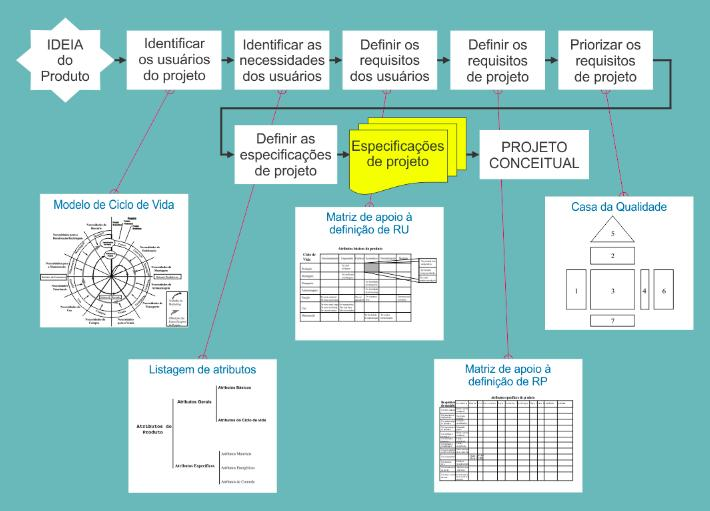
\includegraphics[width=\textwidth]{pictures/1180.jpg}
	\end{center}
	\fonte{\autocite{PRODIP}}
\end{figure}

No final do projeto informacional, é obtido de maneira clara e organizada quais são os requisitos do cliente em relação ao produto que está em desenvolvimento e quais são as
funções o produto necessários que o produto necessita ter a fim de realizar os requisitos do cliente.
Também se obtém, de forma quantizada, a ordem de prioridade nas quais o projeto necessita realizar os requisitos.

\subsection{Projeto conceitual}

Nesta etapa do projeto inicia-se o projeto e desenvolvimento das soluções conceituais para se atingir os requisitos obtidos na etapa anterior, o projeto conceitual é
caracterizado pela fase criativa onde são geradas e avaliadas técnica e economicamente as alternativas para resolução do problema.
As principais ferramentas utilizadas no projeto conceitual são mostradas na \autoref{fig:1190} e dentre elas se destacam matriz síntese de funções, matriz morfológica
e matrizes multi critério de seleção \autocite{PRODIP}.

\begin{figure}[htb]
	\caption{\label{fig:1190}Etapas do projeto conceitual}
	\begin{center}
		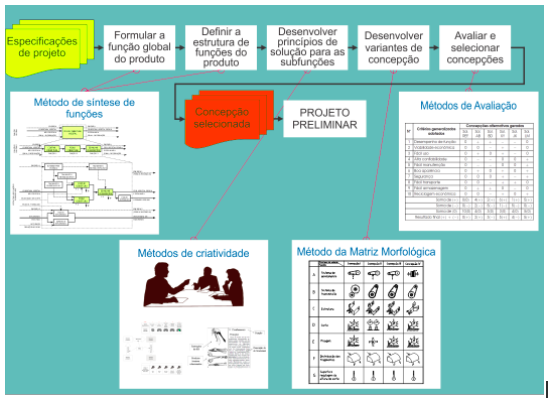
\includegraphics[width=\textwidth]{pictures/1190.png}
	\end{center}
	\fonte{\autocite{PRODIP}}
\end{figure}

\subsection{Projeto preliminar}

No projeto preliminar é definido a forma final do produto, nessa fase são definidas características geométricas, de montagem, materiais para fabricação, características
ergonômicas e de segurança e processos de manufatura do produto. Também pode ser realizados testes com protótipos para prova de conceito e otimização das características
do produto desenvolvido até essa fase. \autocite{Back2008}

Os resultados dessa fase são as documentações de viabilidade econômica e requisitos de manufatura, e um protótipo funcional do produto.

\subsection{Projeto detalhado}

A elaboração do projeto detalhado se destina a vários propósitos, como a aprovação do protótipo, a finalização das especificações dos componentes e o detalhamento do plano
de manufatura \autocite{Back2008}.

Nessa fase são gerados as documentações de especificação dos componentes, como desenhos técnicos, esquemas elétricos, planos de manufatura e softwares utilizados. Nesta fase
são feitos testes em campo e laboratório e acontece a otimização do protótipo com objetivo de preparação para produção.
